\subsection{Related Standards}
\paragraph{C++20} C++ will be programmed according to the C++20 standard, formally known as
\href{https://www.iso.org/standard/79358.html}{ISO/IEC 14882:2020}. C++ is
a superset of C, and builds upon it by introducing object-oriented
programming concepts while maintaining the functional language aspect of C.

\paragraph{802.11} The microcontroller (MCU) supports transmission through the Institute of
Electrical and Electronics Engineers (IEEE) 802.11b/g/n standard of wireless
communication. This standard uses the S band of radio frequences and
operates at 2.4 GHz. There are 14 accessible channels, each spanning a band
width of 22 MHz (pictured in\autoref{wifi_channels}).
\begin{figure}[H]
    \caption{802.11b/g/n channels}
    \label{wifi_channels}
    \centering
    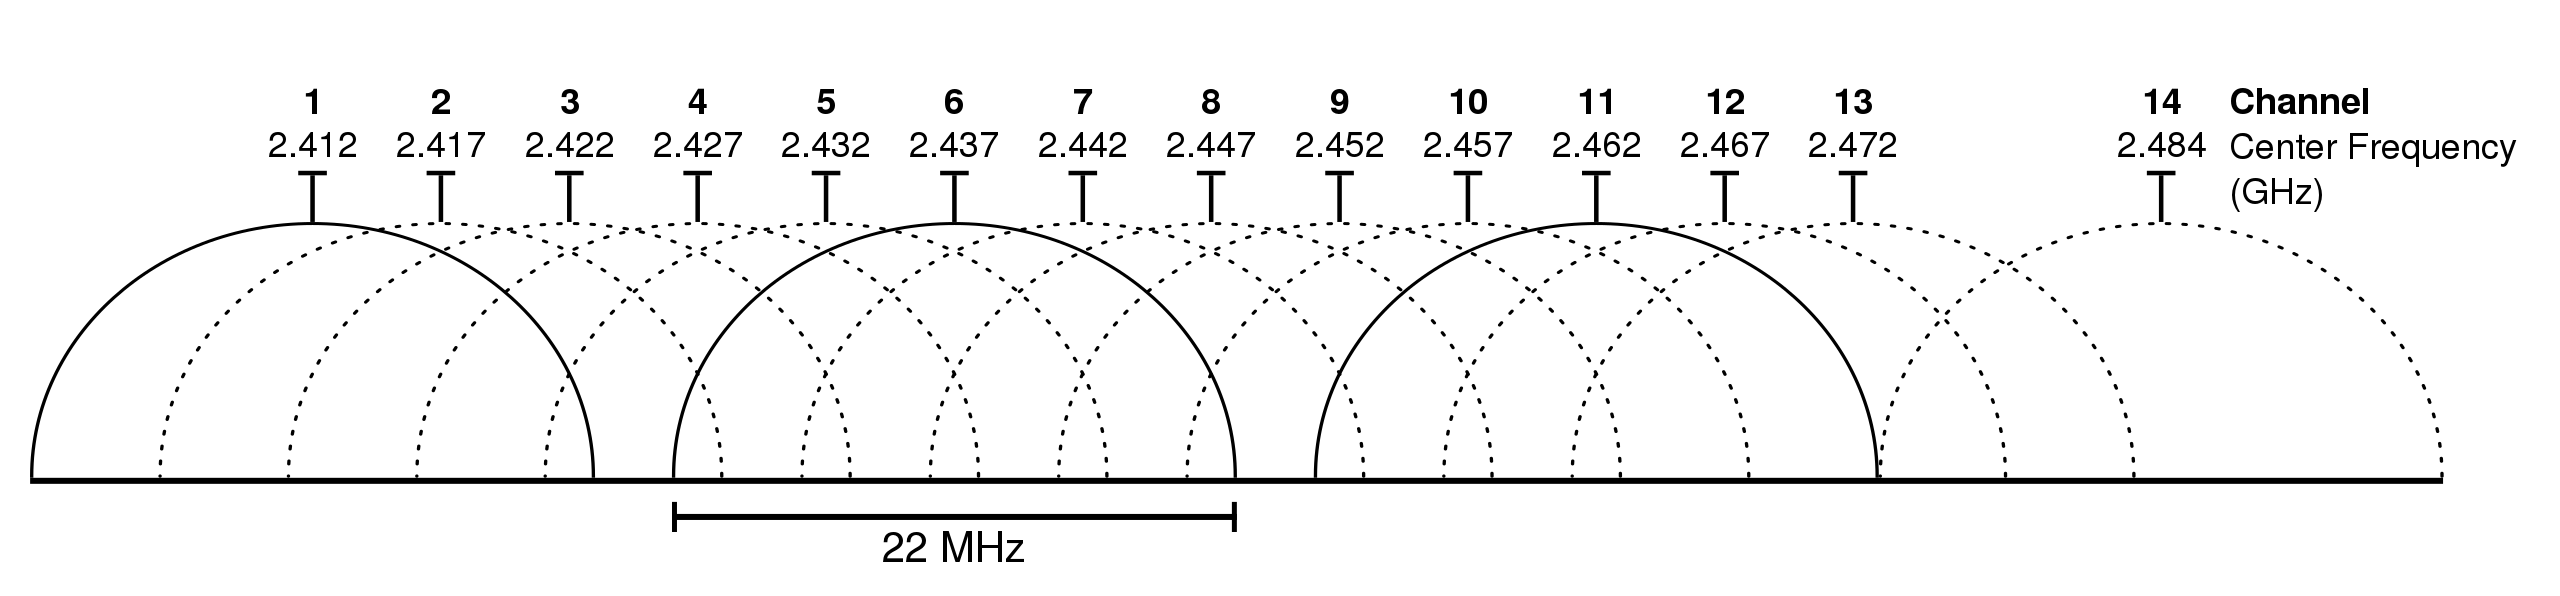
\includegraphics[width=0.75\textwidth]{images/wifi_channels.png}
\end{figure}
These channels specifically reside in an industrial, scientific and medical
(ISM) band. This standard also provides datagram frames for the transport
layer.

\paragraph{TCP} \label{tcp_standard} Transmission Control Protocol (TCP) will be used to satisfy transport layer
requirements of the product, and will be used to transmit symbols (i.e.
from any commands, data, settings, telemetry, etc.) between Amazon Web
Services (AWS) and the microcontroller (MCU). TCP was chosen over other
protocols, such as User Datagram Protocol (UDP), mainly due to its
reliability. The extent of TCP's reliability includes features such as
checksums, duplicate data detection, retrying of transmissions, sequencing,
and timers.
Such reliability is favored over higher bandwidth or lower
latency, as neither of the latter are required for the kilobytes
of information being relayed between AWS and the MCU. A standard TCP frame
is shown in \autoref{tcp_frame}.
\begin{figure}[H]
    \caption{TCP frame (\href{https://condor.depaul.edu/jkristof/technotes/tcp.html}{The Transmission Control Protocol}, Fig. 1)}
    \label{tcp_frame}
    \centering
    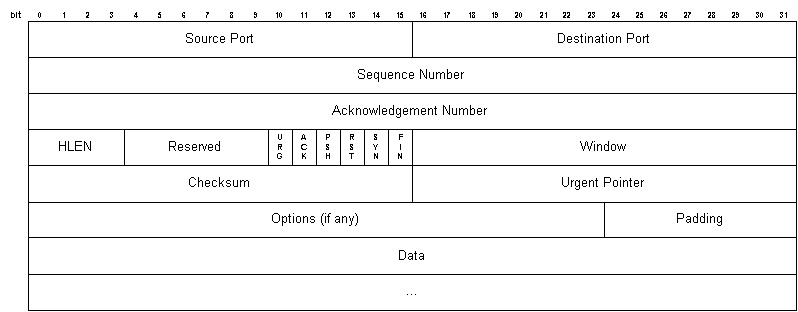
\includegraphics[width=0.75\textwidth]{images/tcp_frame.jpg}
\end{figure}

% TODO TBD
\paragraph{IPv4} TBD. 



\subsubsection{JSON Web Token (RFC 7519)}
This standard specifies a ``compact, URL-safe means of representing claims to be transferred between two parties.'' The means is via the JSON Web Token (JWT). JWTs are split into 3 parts, the header which specifies the algorithm the key(s) used to encrypt the message and the type of token, JSON Web Encryption (JWE) or JSON Web Signature (JWS). The second part is the payload. The payload is a JSON formatted object which carries claims. And the third part is the verification signature which is the Base64 encoded header plus a `.' plus the Base64 encoded payload, another `.' and finally this is all encrypted by the key. When a JWT is received, the header and payload can be read by just Base64 decoding these portions of the token. The JWT is verified by decrypting the verification signature, if the signature cannot be decrypted with the key then the token is invalid. \autoref{fig:jwt} gives an example of a JWT that is signed with a secret key.
\begin{figure}[H]
\centering
\caption{Example JWT from jwt.io}
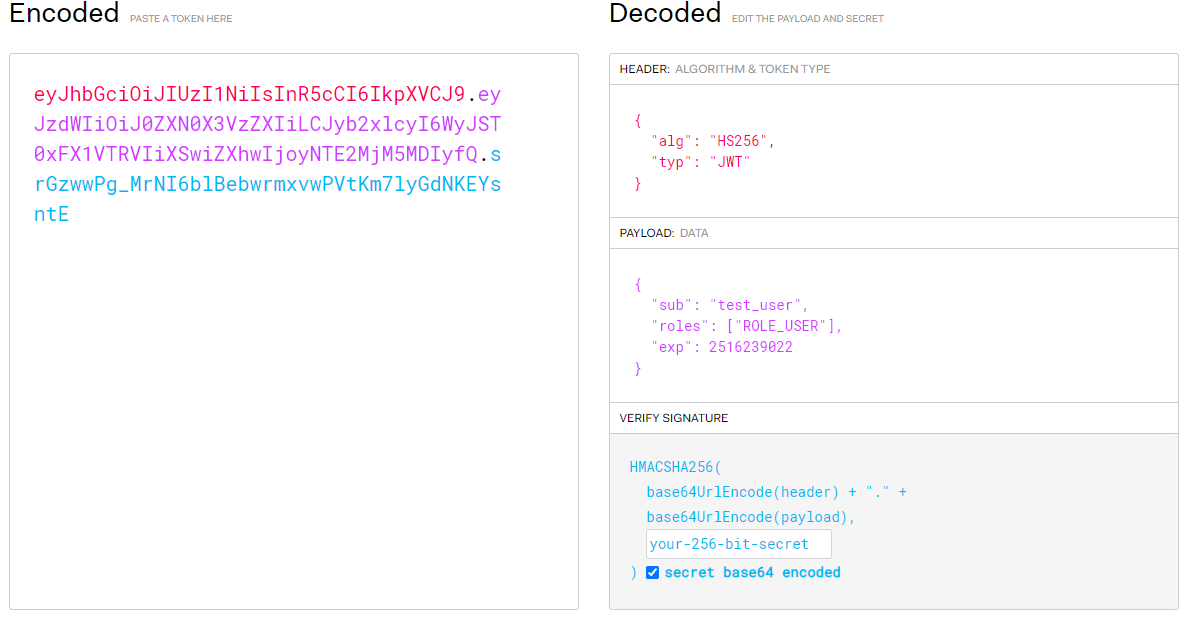
\includegraphics[width=\textwidth]{images/jwt.png}
\label{fig:jwt}
\end{figure}

\paragraph{Claims}
Claims are in the payload of a JWT. The basic claims specified by this standard are \verb|iss| ``issuer'', \verb|sub| ``subject'', \verb|aud| ``audience'', \verb|exp| ``expiration'', \verb|nbf| ``not before'', \verb|iat| ``issued at'', and \verb|jti| ``JSON Token ID''. For our purposes, all of the JWTs will be self-signed so the issuer, JSON Token ID, audience, and issuer claims can all be disregarded as they are meant for cross-service authentication. However, following the standard, the ``subject'' claim will be the user principal, and the expiration and issuad at claims will be used to invalidate a token cookie after a certain period of time. The standard allows for public and private claims outside of these as well. Public claims are registered with the IANA while private claims are collision prone, neither of these are of true concern to us.
\subsubsection{HTTP/1.1 (RFC 2616)}
This standard defines an application-level protocol communicating across the internet. RFC 2616 is an update to previous protocols that increase the capabilities of the original in the form of persistent connections and the ability to send files in the form of MIME types. MIME types hold metadata and the binary data of a file. This standard also serves to define how dates/times are handled on the web as well.
\subsubsection{WebSocket Protocol (RFC 6455)} \label{websocket_protocol}
The WebSocket Protocol standard is important to frame the way that the web server and microcontroller communicate. It specificies how the connection is made, how the data is formatted, and some security considerations. Most of these items are abstracted away from users in the forms of libraries however the security concerns are likely the most important part of this standard in terms of this project. The reason being that we are receiving location and IP data from the packets in order to build out commands like where to point the solar panels. Exposing PII such as location to the world wide web is a major concern that we would like to avoid by following this standard.